\documentclass[en]{../../../../../../eplexam}

\usepackage{../../../../../../eplunits}
\usepackage[american]{circuitikz}
\usepackage{bm}

\hypertitle{Power Electronics}{7}{ELEC}{2660}{2019}{Janvier}{All}
{Martin Braquet \and Louis Fichefet \and Clément Martin}
{Marc Bekemans}

\section{Expliquez ce slide (contexte, explications détaillées, équations, \dots)  /4}

\begin{figure}[h!]
    \centering
    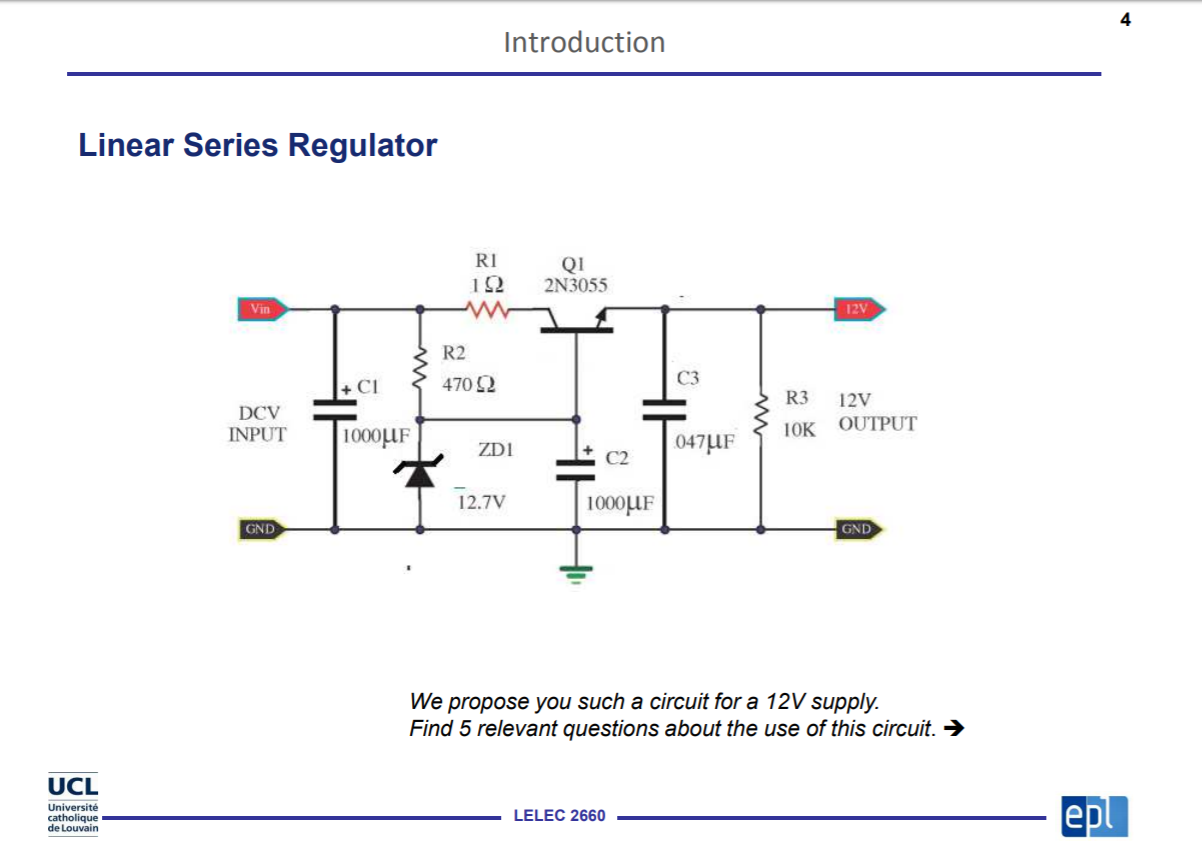
\includegraphics[scale=0.5]{Q1.png}
\end{figure}

\nosolution

\section{Expliquez ce slide (contexte, explications détaillées, équations,\dots)  /4}

\begin{figure}[h!]
    \centering
    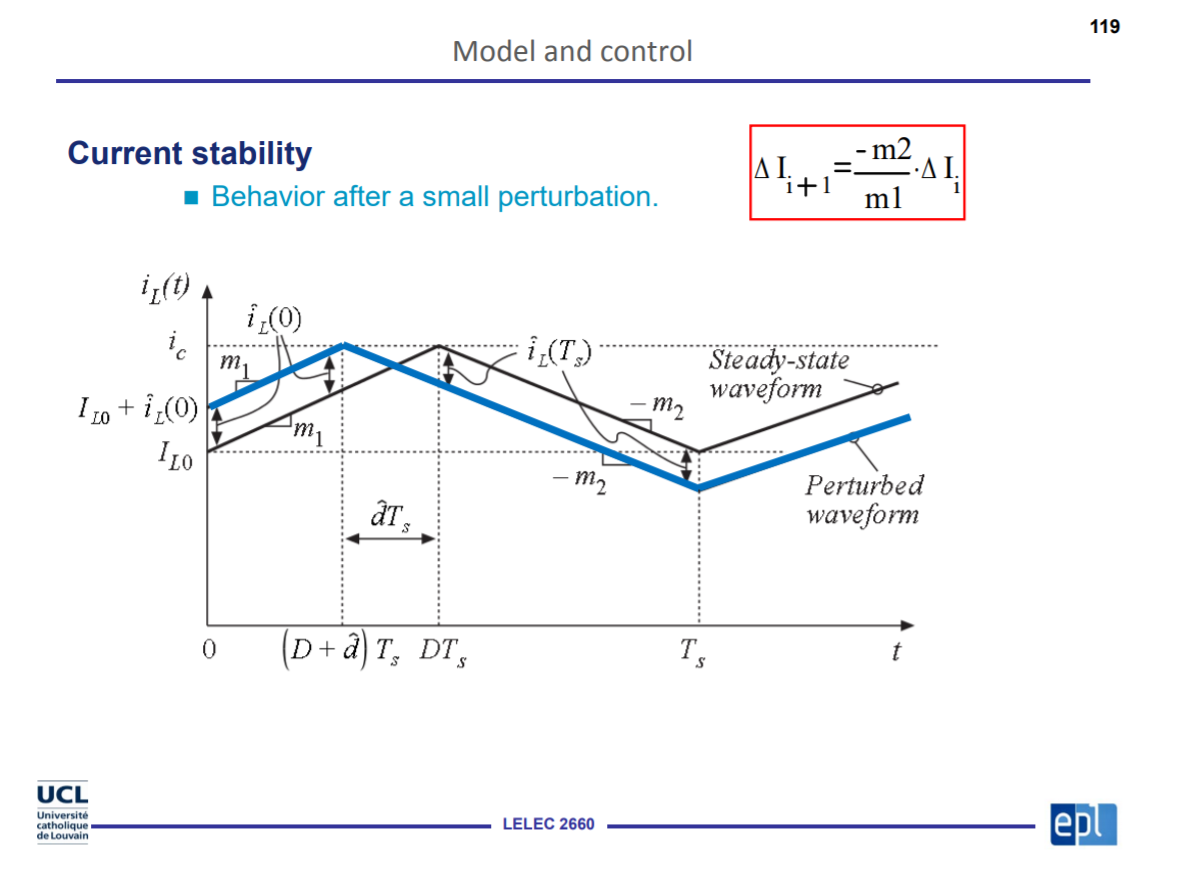
\includegraphics[scale=0.5]{Q2.png}
\end{figure}

\nosolution

\section{Série de questions rapides  /16}

\begin{itemize}
    \item En mode bloqué, un IGBT bloque les tensions dans les deux sens. Vrai/Faux.
    \item Soit un convertisseur Flyback. Quelles sont les conséquences au fait de doubler l'entrefer ?
    \item Soit un redresseur en bialternance connecté à une charge résistive avec une tension de 50 V DC à ses bornes. On décide de remplacer la charge par une capacité. Quelle est la tension à ses bornes ?
    \item Soit un redresseur triphasé non commandé à 6 diodes et alimenté par du 50 Hz. Quelle est la fréquence de la fondamentale de la tension de sortie ?
    \item Dans le peak current control, la condition de stabilité est que le rapport cyclique ne dépasse pas 50 \%. Vrai/Faux.
    \item Une diode avec les caractéristiques suivantes : $V_f = 850$ mV, $R_{th_{j-C}}$ = 0.15 K/W est parcourue par un courant de 50 A pendant 30 \% du temps sur une période. Sachant que l'air ambiant est à \SI{25}{\celsius} et que la température de jonction de la diode ne peut pas dépasser \SI{100}{\celsius}, quelle doit être la résistance thermique du radiateur ?
    \item Soit un convertisseur Buck avec les caractéristiques suivantes : $V_o$ = 25 V, $V_i$ = 100 V, $f_{SW} = \SI{100}{kHz}$, $L = \SI{250}{\micro H}$, quelle est la puissance de sortie minimale requise ?
    \item Écrivez l'équation du transfert de puissance complexe entre deux sources de courant alternatives $U_1$ et $U_2$ liées par une inductance $L$.
\end{itemize}

\nosolution

\section{Exercice  /4}

On considère un Boost avec les caractéristiques suivantes :
\begin{itemize}
    \item $V_{in}$ = 50 V
    \item $V_{out}$ = 100 V
    \item $L = \SI{500}{\micro H}$
    \item $f_{sw}$ = 100 kHz
    \item $P_{out}$ = 100 W
\end{itemize}
Déterminez le nombre de capacités ($C = \SI{100}{\micro F}$, $r = \SI{100}{m\Omega}$) mises en sortie pour que le ripple de la tension de sortie ne dépasse pas $150$ mV (peak to peak).

\nosolution

\section{Question de théorie  /6}
    
On considère ici un convertisseur Flyback dans lequel on a rajouté un \textit{snubber}\footnote{Le \textit{snubber} a été vu en séance d'exercice sous la forme d'un projet dédié à la conception d'un transformateur.}. Expliquez le fonctionnement du snubber et comment choisir ses composants. Commentez, dessinez les formes d'ondes, schémas, etc.

\nosolution

\section{Superbuck  /6}

Soit le convertisseur suivant :

\begin{center}
	\begin{circuitikz}
		\draw[thick]
		(0,0) node[nmos, rotate = 90](nmos){}
		(nmos.D) to[short] (-2,0)
		(nmos.S) to[short] (5,0)
		(1.5,-2) to[diode] (1.5,0)
		(-1.5,-2) to[short] (1.5,-2)
		(-4,0) to[american voltage source,a=$V_{\mathrm{g}}$,right] (-4,-4) -- (5,-4)
		(5,0) to[R, l_=$R$, v^=$V$] (5,-4)
		(-4,0) to[L=$L$] (-2,0)
		(3,-4) to[C=$C$] (3,0)
		(0,-4) to[L=$L$] (0,-2)
		(-1.5,-2) to[C=$C$] (-1.5,0);
	\end{circuitikz}
\end{center}

Écrivez la matrice dynamique des états moyennés $\bm{A}$, en fonction du rapport cyclique.

\nosolution

\end{document}
